\documentclass{article}

\title{SEED Lab Mini Project Team 3 Documentation}
\author{
    Dawson J. Gullickson
    \and
    Julia Kaase
    \and
    Nick Nijkamp
    \and
    Sam Leonard
}
\date{\today}

% \usepackage{amsmath}
\usepackage{geometry}
\usepackage{hyperref}
\usepackage{graphicx}
\usepackage{listings}
% \usepackage{multicol}
\usepackage{xcolor}

% Margins (geometry)
\geometry{margin=1in}

% Code Styling (listings, xcolor)
\definecolor{mygreen}{rgb}{0,0.6,0}
\definecolor{mygray}{rgb}{0.5,0.5,0.5}
\definecolor{mymauve}{rgb}{0.58,0,0.82}
\lstset{
    basicstyle=\footnotesize,
    commentstyle=\color{mygreen},
    keywordstyle=\color{blue},
    stringstyle=\color{mymauve},
    numbers=left,
    breaklines=true,
    showstringspaces=false,
}

% No page numbers
\pagenumbering{gobble}

\begin{document}
    \maketitle
	
    \begin{enumerate}
        % 1
        \item The computer vision part of this mini project is run on a raspberry pi. In the code, we have a function called \verb|video()|, which does all the computer vision part of the project. \verb|video()| uses open cv to capture the camera output, which is called in an infinite loop. We convert the image to grayscale, as it is more reliable in reading the aruco markers that way. We add the library of markers, and then if we have 1 or more corners detected, we know we have a marker in the frame. When we have a marker on the frame, we sum up all the x-axis corner values and average them out by dividing by 4. We do the same for the y values. This give is the middle of the marker. The frame outputs in a roughly 473x635 frame. So with some simple if else logic, we can take half of these max x and y values to see if we are in a certain quadrant. For example, if the \verb|xMiddle > 318| and \verb|yMiddle < 237|, we know that we are in quadrant 1 (top right). We set a variable called \verb|quadrant| equal to 1, 2, 3, or 4 so that can be passes along to the Arduino. If there are no markers on the screen, \verb|quadrant == 0|.
        
        % 2
        \item \ \\
        \begin{center}
            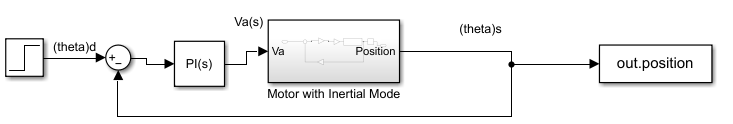
\includegraphics[width=0.8\linewidth]{closedLoop.PNG}
        \end{center}
        Below is the closed loop step response graph generated from the motor.
        \begin{center}
            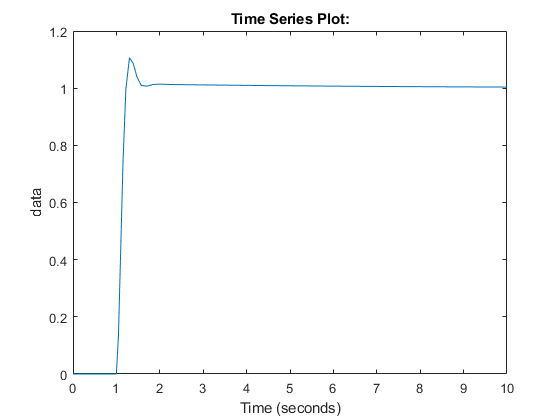
\includegraphics[width=0.6\linewidth]{closedLoopResponse.png}
        \end{center}
        Here is the experimental data generated from the closed loop PI controller:
        \begin{center}
            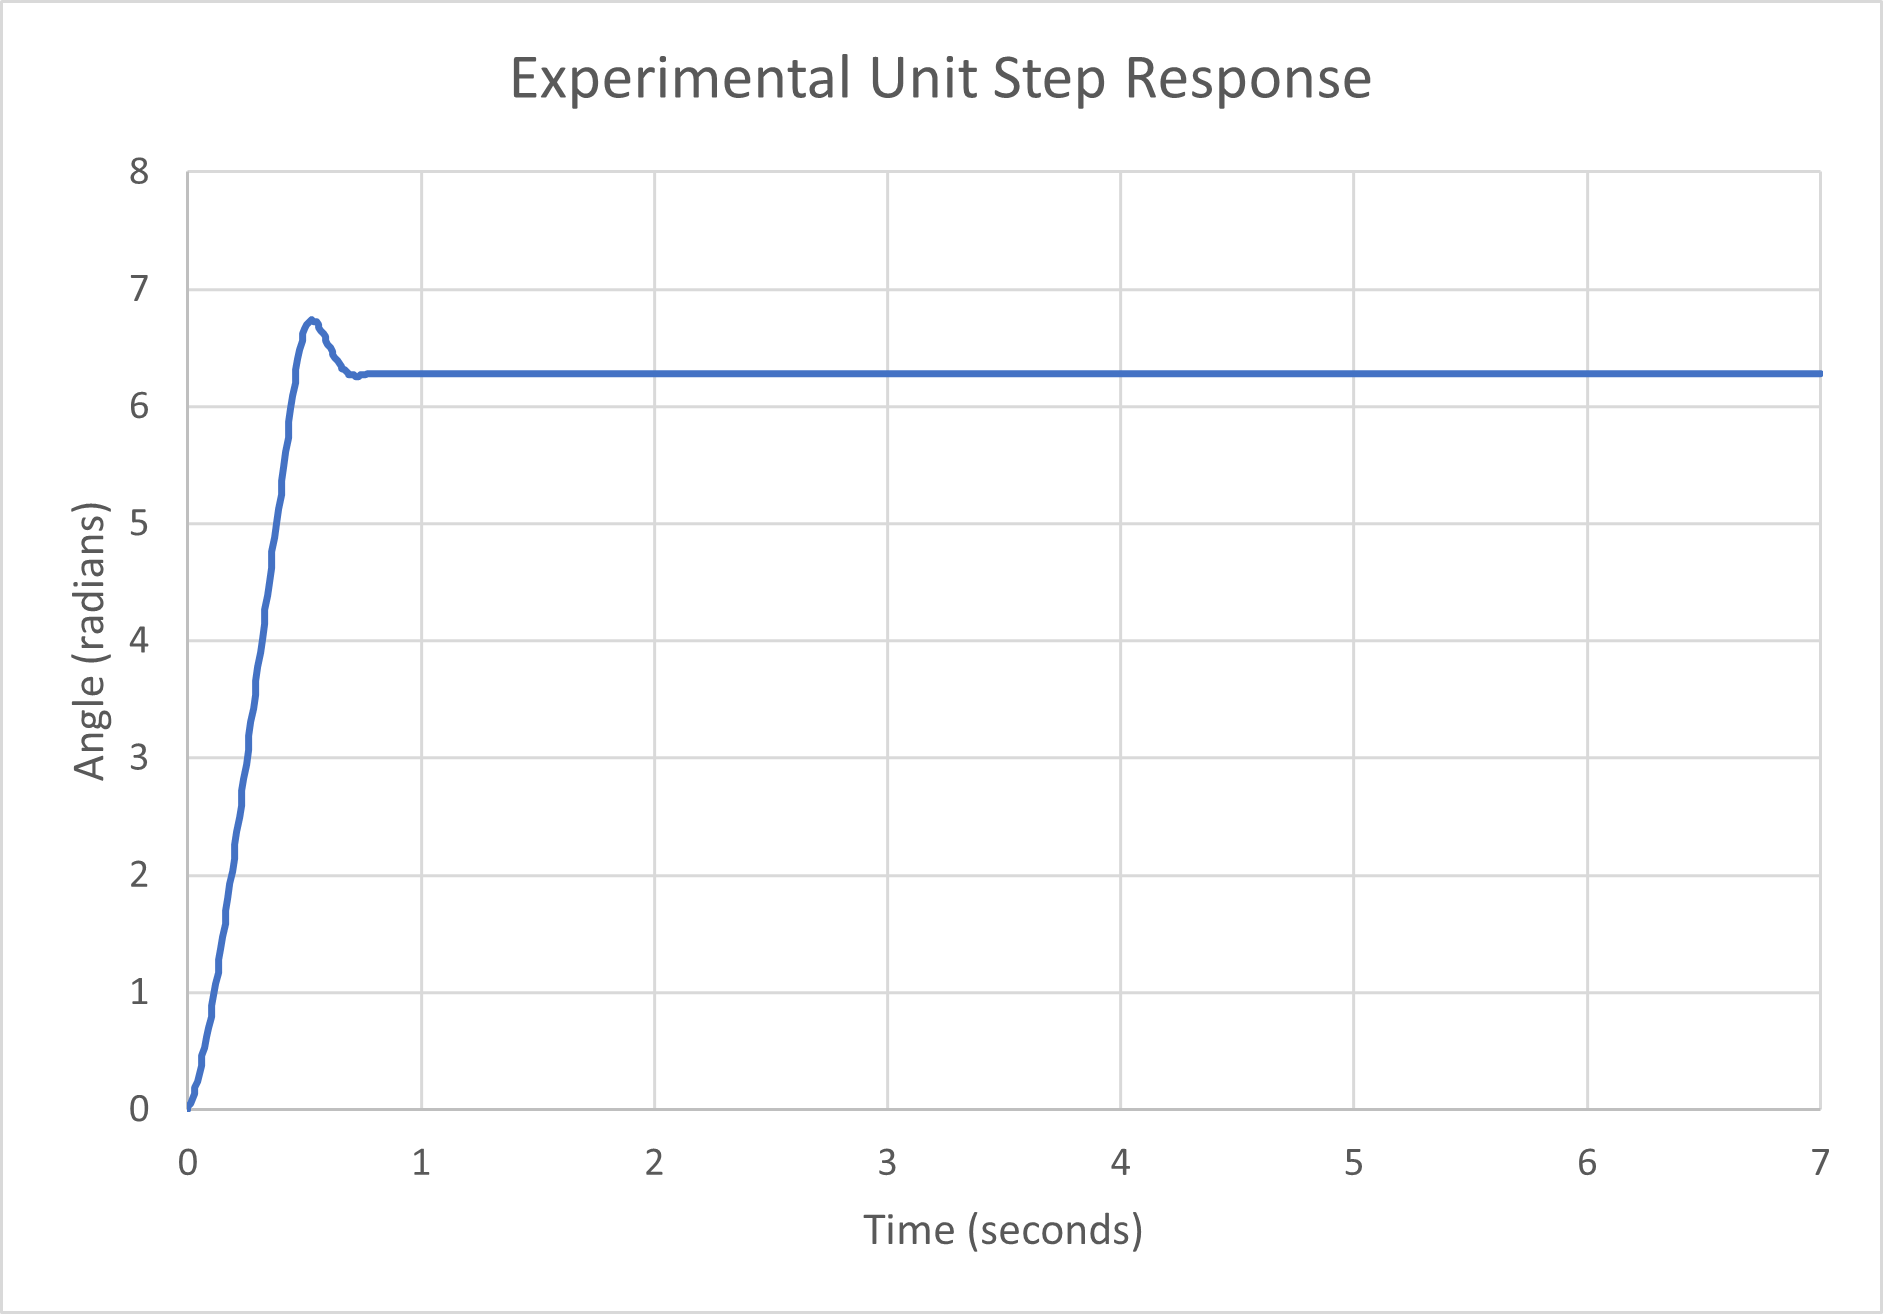
\includegraphics[width=0.6\linewidth]{experimentalClosedLoopResponse.png}
        \end{center}
        The closed loop resoponse adjusts well for overshoot and undershoot. The feedback allows for the motor to maks adjustments as needed. 

        Below is the open loop step response graph generated from the motor.
        \begin{center}
            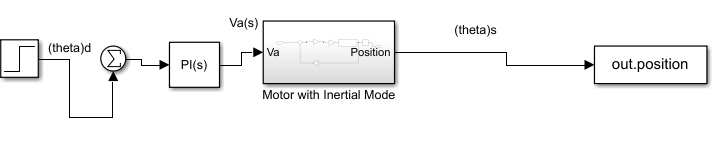
\includegraphics[width=0.8\linewidth]{openLoop.PNG}
        \end{center}
        Implementing the open loop response would not work well, the motor goes off to infinity, and does not keep track of where it should be. 
        \begin{center}
            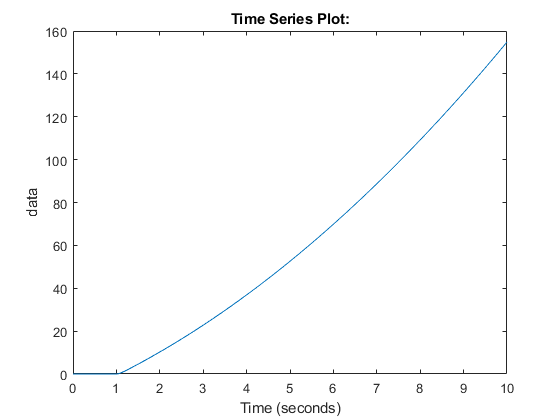
\includegraphics[width=0.6\linewidth]{openLoopResponse.png}
        \end{center}
        % 3
        \item Arduino Code:
        \subitem PID Variables:
        \begin{lstlisting}[language=C++]
double Kp = 15.3786175942488; // V/rad
double Ki = 2.37803426483209; // V/(rad*s)
double Kd = 0;                // V*s/rad
        \end{lstlisting}
        \subitem Controller Code:
        \begin{lstlisting}[language=C++]
// calc error
double e = r-y; // find where it needs to move from where it is

if (Ts > 0) {
    D = (e-e_past)/Ts; // derivative
    e_past = e; // update val to get other vals
} else {
    D = 0;
}

I = I+Ts*e; // integral

// Calc controller output -- output voltage uses PID
double u = Kp*e+Ki*I+Kd*D;
// deals with actuator saturation
// i.e. if trying to write a voltage too high for board to supply
if (abs(u) > umax) {
    u = sgn(u)*umax;
    e = sgn(e)*min(umax/Kp, abs(e));
    I = (u-Kp*e-Kd*D)/Ki; 
}

// Convert voltage to speed
int speed = -u*400/umax;
        \end{lstlisting}
        \begin{center}
            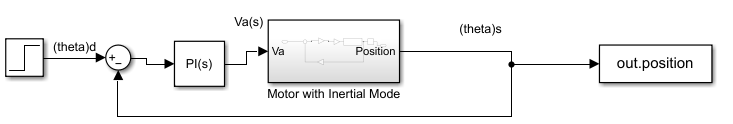
\includegraphics[width=0.8\linewidth]{closedLoop.PNG}
        \end{center}

        % 4
        \item Github repository: \url{https://github.com/nrnijkamp/SEEDLab}
    \end{enumerate}
\end{document}